\documentclass[12pt]{article}

% --- Encoding & basic fonts -----------------------------------------
\usepackage[utf8]{inputenc}
\usepackage{lmodern}

% --- Core tools -----------------------------------------------------
\usepackage{xparse}           % needed for \IfValueT (kept; harmless)
\usepackage{enumitem}         % custom lists

% --- Layout, colour, graphics ---------------------------------------
\usepackage{geometry}
\usepackage{xcolor}
\usepackage[most]{tcolorbox}
\usepackage{graphicx}         % enable images (needed for logo)

% --- Long-table & hyperlinks ----------------------------
\usepackage{longtable}
\usepackage{hyperref}
\usepackage{bookmark}         % better PDF outlines

% --- Typography & line breaking helpers -----------------
\usepackage[final]{microtype}
\emergencystretch=2em

\geometry{margin=1in}
\hypersetup{
  colorlinks  = true,
  linkcolor   = blue,
  urlcolor    = blue,
  pdftitle    = {System Requirements Specification},
  pdfpagemode = FullScreen,
}
% must be loaded after hyperref!
\usepackage{cleveref}
\usepackage{amsmath}

% ===================================================================
%                       MOSCOW PRIORITY TAGS
% ===================================================================
\newcommand{\PriorityTag}[2]{%
  \colorbox{#2!25}{\footnotesize\textsf{\textbf{#1}}}\hspace{0.6em}}

\newcommand{\must}{\leavevmode\PriorityTag{Must}{green}}
\newcommand{\should}{\leavevmode\PriorityTag{Should}{yellow}}
\newcommand{\could}{\leavevmode\PriorityTag{Could}{cyan}}
\newcommand{\wont}{\leavevmode\PriorityTag{Won't}{red}}

% ===================================================================
%                       Requirements box
% ===================================================================

% Make hyperref anchors for requirement numbers unique across groups/sections.
% Keep this AFTER hyperref is loaded (above).

\newcounter{reqgrp}[section] % one group per section; change parent if desired
\renewcommand{\theHreqno}{\thesection.\arabic{reqgrp}.\arabic{reqno}}


\newcounter{reqno}
\newcommand{\reqprefix}{GEN}

\newif\ifshowverification
\showverificationfalse % flip to \showverificationtrue to show Verification lines

\newcommand{\reqnum}{%
  \ifnum\value{reqno}<10 0\fi
  \ifnum\value{reqno}<1 00\fi
  \arabic{reqno}%
}

\newenvironment{requirements}[1]{%
  \renewcommand{\reqprefix}{#1}%
  \refstepcounter{reqgrp}% start a new anchor group per block
  \setcounter{reqno}{0}%
  \begin{enumerate}[leftmargin=*]
}{\end{enumerate}}

\makeatletter
% \req{Title}{Shall-statement}{Acceptance}[Verification]
\NewDocumentCommand{\req}{m m m O{}}{%
  \refstepcounter{reqno}%
  \protected@edef\@currentlabel{REQ-\reqprefix-\reqnum}%
  \textbf{REQ-\reqprefix-\reqnum\ -- #1.} #2\par
  \emph{Acceptance:} #3\par
  \if\relax\detokenize{#4}\relax\else
    \emph{Verification:} #4\par
  \fi
}
\makeatother

% ===================================================================
%                       Title metadata
% ===================================================================

\newcommand{\CompanyLogoPath}{images/asi-logo.png}

\title{4D-STEM Requirements Specification}
\author{Ciaran Welsh / SEM Team}
\date{\today}



\begin{document}

\maketitle

\begin{center}
  
\includegraphics[width=0.5\textwidth]{asi-logo}
\end{center}

\tableofcontents
\newpage


\section{Introduction}\label{sec:intro}
% Purpose - who is the product for?
This document defines the implementation-independent software requirements for 4D-STEM users. It is a living reference for software and application engineers as well as the business teams at ASI. The document should be considered a `living document' that should be updated in an organized manner as the project evolves.

4D-STEM (Four Dimensional Scanning Transmission Electron Microscopy) is a microscopy technique where a focused electron beam is scanned across a sample, producing a 2D diffraction pattern at each position. The resulting four-dimensional dataset, with two spatial and two reciprocal-space dimensions, enables detailed analysis of structure, strain, and other material properties. The advantage that Timepix3 (and Timepix4) offer such an application are derived from the event-driven nature of the detector; timepix detectors record each electron hit independently from other pixels which avoids some of the frame-based limitations and offering greater performance. This also allows small dwell times, improves dose efficiency for beam-sensitive samples, reduces data volume through sparse readout, and supports real-time analysis with lower memory and bandwidth requirements.

% project scope - overview of the product in relation to business goals. What are the expected outcomes?
ASI specializes in Timepix3 and now Timepix4 detectors, and this project aims to deliver a complete 4D-STEM solution, not just the detector hardware. The software will enable customers to control their detectors, acquire data, and process it in real time, forming a cohesive package for scientists conducting 4D-STEM experiments. The solution aims to be primarily acquisition software; any processing conducted by the software should adhere to the goal of enabling 4D-stem application scientists acquire data for further processing in whatever tool they choose. The solution will replace the current 4D-STEM features in Serval and Accos, simplifying both of them and separating out the responsibilities of 4D-STEM and other application areas.

The primary business goal is to increase adoption of ASI detectors by providing a specialised, high-performance 4D-STEM platform that reduces user complexity and enables 4D-STEM research workflows. Success will be defined by users being able to control both their scan engine and Timepix device from a single UI, conduct experiments without performance issues, and view processed results in real time without needing to manage the data pipeline themselves. Finally they should be able to export data in ways useful to their further analysis, for example in LiberTEM, HyperSpy and py4dStem.

The software will focus on 4D-STEM workflows, with possible inclusion of 4D-STEM EELS in the future. It will not support ptychography, conventional STEM or general detector control, which are explicitly out of scope. For the latter, users can use Accos or Serval directly.

\subsection{Definitions and Acronyms}
% Clearly define all key terms, acronyms, and abbreviations used in the SRS. This will help eliminate any ambiguity and ensure that all parties easily understand the document.
\begin{enumerate}
    \item CBED
    \item vADF
    \item iDPC
    \item iCOM
\end{enumerate}


\section{Overall Description}\label{sec:overall_description}
% Purpose: Provide a high-level view of the product and boundaries before detailed requirements.
% Guidance: Keep technology-agnostic and avoid "shall" statements in this section.
This product is a dedicated 4D-STEM acquisition application designed for ASI's Timepix3 and Timepix4 detectors. It provides an integrated environment for configuring experiments, acquiring event data, generating real-time preview images, and exporting results for external analysis. It replaces the 4D-STEM functionality currently in Serval and Accos, separating 4D-STEM acquisition workflows from general detector control and processing.

The application runs on a single workstation together with Serval for detector control and scan-engine control software for communication with the scan generator. Serval configures the detector and streams raw binary event data, which the application processes for display and measurement. The software handles the integration between scan engine and detector and presents results to the user with acquisition statistics and metrics. A general overview of the application’s position in the broader tool ecosystem is shown in \cref{fig:general_structure}.

External connections are:
\begin{itemize}
    \item \textbf{Serval}: REST API for detector configuration and TCP stream for event data.
    \item \textbf{Scan generator}: Controlled via vendor-supplied binary (FFI) or gRPC.
    \item \textbf{Local storage}: High-throughput NVMe drives for data capture.
\end{itemize}

\begin{figure}[t]
    \centering
    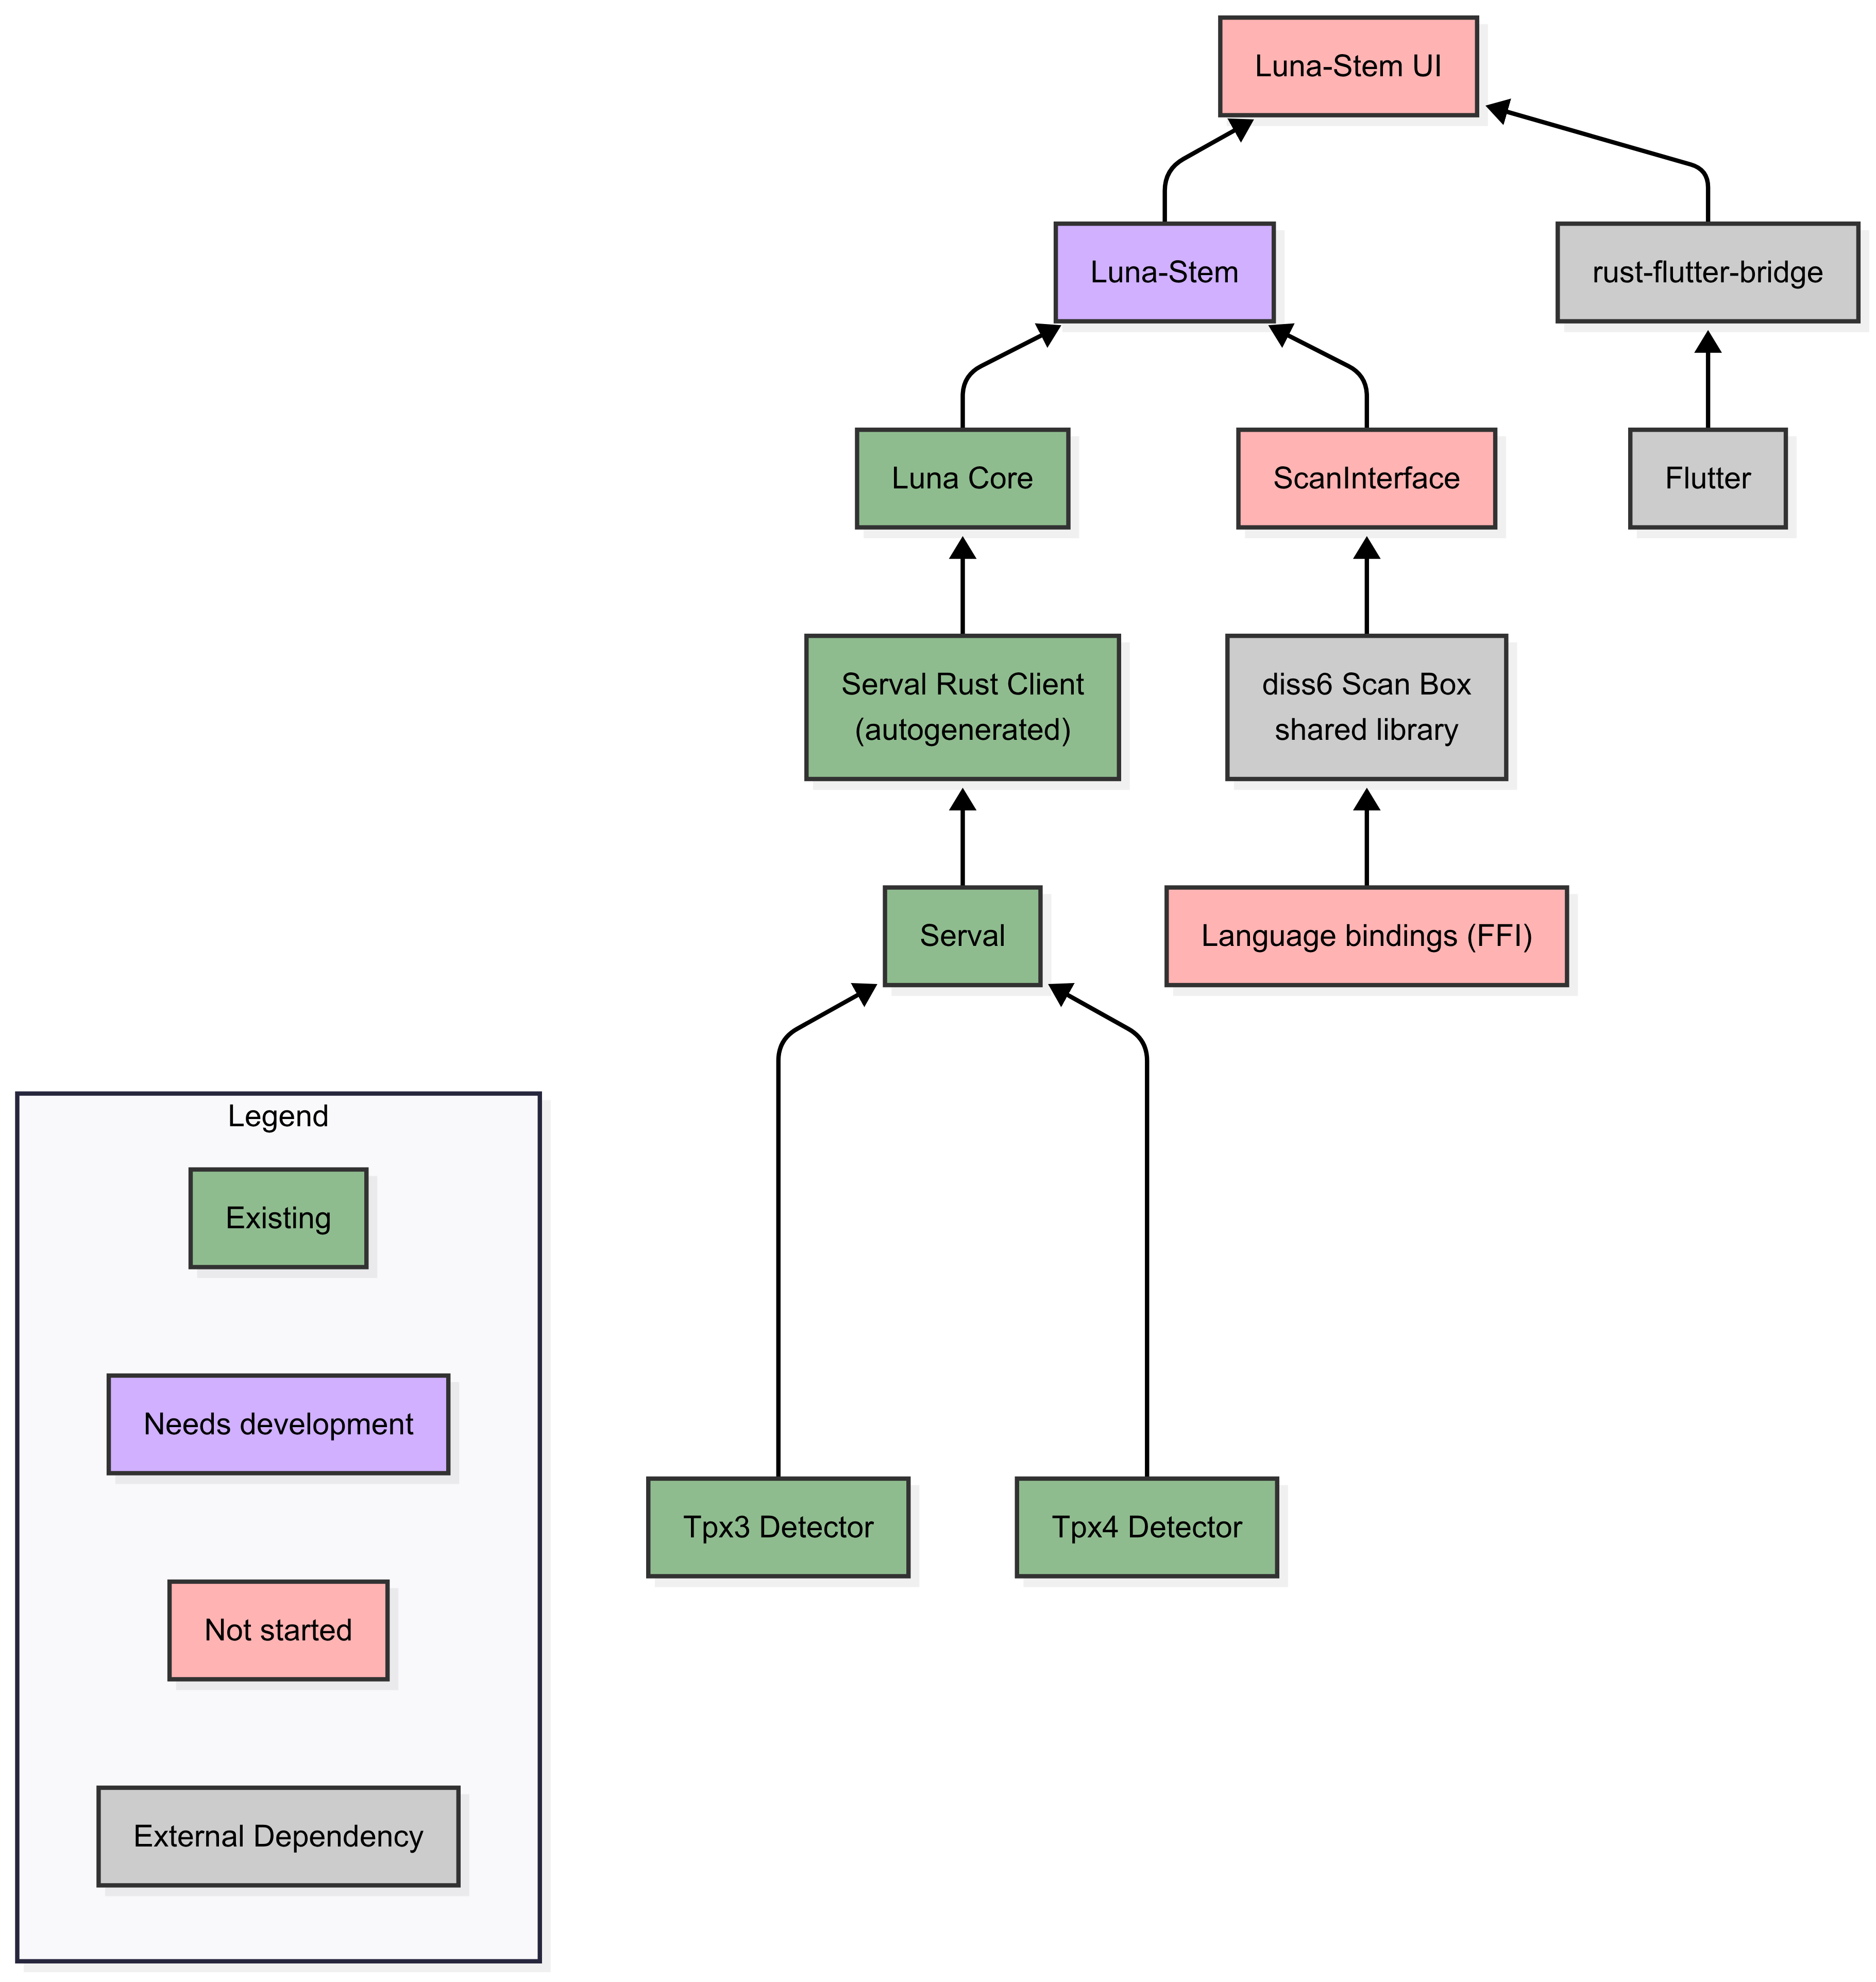
\includegraphics[width=0.7\linewidth]{GeneralStructure}
    \caption{Overview of the application in relation to other tools}
    \label{fig:general_structure}
\end{figure}


\subsection{User Classes and Characteristics}\label{subsec:user-classes-and-characteristics}
% Purpose: Describe user groups and relevant characteristics that affect design and UX.
% Guidance: Do not list needs here; needs belong in Section 2.6.
The primary users are 4D-STEM scientists, who also operate the microscope. Users range from computationally literate power users to those without much experience. Both users are mainly focused on scientific outcome rather than on the processing required to get them there. The software abstracts data acquisition and visualisation details so that no programming skills are required. All functions are available without special permissions.

\subsection{Operating Environment}\label{subsec:operating-environment}
% Purpose: Define hardware, OS, network, and site constraints that impact design and testing.
% Guidance: Include only factors that materially constrain architecture or verification.
The application supports Windows, Ubuntu, and macOS at launch; other Linux distributions can be built on request. It runs on high-performance lab workstations with specifications sufficient for sustained high-rate data capture and processing. GPU acceleration is planned for future versions but is not required initially. The system operates on localhost only, with all components running on the same machine. Storage must sustain the highest practical write speeds for the selected output format.

\subsection{User Needs}\label{subsec:user-needs}
% Purpose: Capture what users are trying to accomplish and why; basis for traceability.
% Guidance: Paste or reference the enumerated needs with rationale; no solutions here.

\subsection{Assumptions and Dependencies}
% Purpose: Record assumptions to monitor and external dependencies that can fail.
% Guidance: Keep items checkable; they become risks if invalidated.

\subsection{User Needs}
% user classes: Describe who will use the software and what are the expectations of the user?
% “User needs” capture the *problem space* (what the people using the product are trying to accomplish) while “Features” capture the *solution space* (what the system will do to meet those needs).} Putting them in separate sections makes it possible to trace every feature back to a genuine user demand and to challenge any feature that has no such lineage.
\begin{enumerate}
  \item \textbf{Dedicated 4D-STEM interface separate from the generic detector UI}\\
        \textit{Rationale: Build with a 4D-stem first mentality. Makes software 4d-stem centric, minimises cognitive load on our users needing to compete with more general use cases and prevents accidental changes to routine detector operations. Separation of concerns.}
  \item \textbf{Immediate, clearly organized access to all scan-generator controls}\\
        \textit{Rationale: Reduces set-up time, enhances usability and ensures detector settings stay consistent with scan parameters.}
  \item \textbf{Seamless integration with Serval for detector control whilst being exposed to only what they need}\\
        \textit{Rationale: Serval must be used for detector control but minimizing the user interaction with Serval reduces the learning curve and enhances usability}
  \item \textbf{Real-time visual feedback during scans}\\
        \textit{Rationale: Enables rapid navigation to regions of interest and immediate quality assessment. Also prevents wasted beam time.}
  \item \textbf{Acquire continuous or multi-frame (“Z-stack”) scans}\\
        \textit{Rationale: Lets users monitor radiation damage frame-by-frame.}
  \item \textbf{Ability to run essential offline analyses inside the application}\\
        \textit{Rationale: Enables quality assessment decisions without exporting large datasets to external tools.}
  \item \textbf{Flexible detector masking (hardware or software) to include/exclude pixels before acquisition.}\\
        \textit{Rationale: Controls data volume and tailor field-of-view after initial acquisition in post-processing.}
  \item \textbf{Interactive pixel group selection for averaged diffraction images}\\
        \textit{Rationale: Users can observe averaged regions of sample in diffraction space.}
  \item \textbf{Switchable scan modes to balance performance and user feedback trade-offs}\\
        \textit{Rationale: When searching for interesting features for capture, we need to optimize performance, and low latency preview. When acquiring data "for real", we optimize data integrity for further analysis.}
  \item \textbf{Export raw \emph{or} processed data in open formats (e.g.\ SparseArray, HDF5, Zarr) and where appropriate, image data}\\
        \textit{Rationale: Guarantees images can be saved and interoperability with analysis suites such as LiberTEM, HyperSpy, and py4DSTEM.}
  \item \textbf{Real-time observability of acquisition-pipeline health (hit-rate, processing load, synchronisation)}\\
        \textit{Rationale: Gives user feedback and "sanity checkibility" for operatives, indicates dropped frames and that hit rate is expected.}
  \item \textbf{Data integrity/fidelity at extreme rates}\\
        \textit{Rationale: Ensures every diffraction event is mapped to the right probe position even in the fastest scans, preserving scientific validity.}
  \item \textbf{Extensibility hooks for future 4D-STEM modalities behind feature flags}\\
        \textit{Rationale: Makes the tool relevant for future and lets advanced users adopt new workflows (e.g.\ EELS, ptychography) without redesigning the core tool.}
  \item \textbf{Possibility to use this tool with Tpx4}\\
    \textit{Rationale: We build for the future now by supporting the next generation Timepix technology from initial design.}
\end{enumerate}


\section{System Features and Requirements}
% What is the system supposed to do? What tasks should it perform? Start with "user need' decompose into atomic functional requirements. Each requirement should be testable.
% Structure :
%   Actor, Action, object and qualifier.
% Functional requirements are system agnostic.


\subsection{Functional Requirements}

\subsubsection{Serval Interaction Layer}
Serval is the control-plane interface between the application and the detector.

\begin{requirements}{SRV}

\item \must \req{Attach or spawn Serval}
  % What should happen
  {On startup, the system shall either (a) attach to a reachable Serval instance at the configured host:port, or (b) spawn Serval as a child process whose lifetime is tied to the 4D-STEM UI.}
  % acceptance criteria
  {Attach succeeds or a child process is started; ownership is recorded in metadata. If attached, the UI does not terminate Serval on exit; if spawned, the UI terminates it cleanly on exit.}
  % test
  [Start with/without reachable Serval. Check attach vs spawn, and exit behavior. Fixture: A mini server that looks like Serval for the parts that matter (dashboard + status).]

\item \must \req{Version negotiation}
  % What should happen
  {On initial connect, the system shall retrieve Serval's API version and compare it to the supported range. If out of range, the UI shall warn; if marked incompatible, operations requiring those features \could be blocked.}
  % acceptance criteria
  {Version captured in logs/metadata; \could correct warning/blocking per compatibility matrix.}
  % test criteria
  [Test: emulate 'too old/too new/incompatible` versions; assert warning banner and \could blocked actions.]

\item \must \req{State subscription (push)}
  % What should happen
  {The client shall subscribe to Serval state changes (e.g., detector \{Disconnected, Connected, Idle, Running\}); \wont periodic polling for state shall not be used.}
  % acceptance criteria
  {State transitions correctly arrive}
  % test criteria
  [Test: push state changes from stub/mock serval; capture timing]

\item \must \req{Detector-connected init sequence}
  % What should happen
  {Upon receiving \emph{detector\_connected}, the system shall perform: (1) upload DACs, (2) upload bad-pixel map (BPC), (3) set data destination, (4) load saved detector settings (e.g. bias) for this detector chipboard Id. Failures stop the sequence and surface a recoverable error.}
  % acceptance criteria
  {All four steps succeed, or the sequence aborts with a clear message; successful steps are idempotent (has no effect) on retry.}
  % test criteria
  [Test: inject failure at each step; assert stop + message; rerun to confirm idempotency of prior steps.]

\item \must \req{Command error model}
  % What should happen
  {All Serval command failures shall be represented or mapped to a structured error with code/type, human message, machine key, and remediation hint.}
  % acceptance criteria
  {Errors in logs and UI contain structured fields; API errors use the documented schema.}
  % test criteria
  [Inspection/Test: trigger known errors; assert schema fields present and logged.]

\item \must \req{Connectivity loss during acquisition}
  % What should happen
  {If the control connection to Serval drops during an active acquisition, the client shall detect loss, attempt reconnect, re-establish subscriptions, and abort the acquisition gracefully.}
  % acceptance criteria
  {Loss detected; after recovery, state is consistent the error is recorded in logs and the user is notified}
  % test criteria
  [Manual test: remove the ethernet cable mid run; verify abort gracefully path. Validate logs.]

\item \must \req{Logging and correlation}
  % What should happen
  {Every Serval command, response, state change, and error shall be logged in the serval http log stored per workspace}
  % acceptance criteria
  {Logs contain request/response pairs}
  % test criteria
  [Send a command; locate the log and validate]

\item \must \req{Transport keepalives}
  % What should happen
  {The client shall use protocol keepalives to detect dead connections without polling for state.}
  % acceptance criteria
  {Dead connections are detected within the configured interval; reconnect attempts follow.}
  % test criteria
  [Test: drop TCP silently; observe keepalive detection timeline and retry behavior.]

\item \must \req{Endpoint configuration}
  % What should happen
  {Serval host, port, and transport shall be configurable in the UI; changes take effect on "accept" button press.}
  % acceptance criteria
  {Editing config changes the target; connections establish to the new endpoint after reconnect.}
  % test criteria
  [Test: change the end point to another socket running a different serval instance. Verify connectivity.]

\item \wont \req{Equalization in client}
  % What should happen
  {The client shall not perform detector equalization; that function remains in Accos.}
  % acceptance criteria
  {No equalization commands exist; UI offers no equalization controls.}

\item \wont \req{Detector orientation in client}
  % What should happen
  {The client shall not manage detector orientation.}
  % acceptance criteria
  {No orientation commands exist; UI offers no orientation controls.}
  % test criteria
  [Inspection.]

\end{requirements}


\subsubsection{Online Image Reconstruction}
\begin{requirements}{OIR}

\item \must \req{Real-time vADF reconstruction}
  % what will be done
  {Raw event data received from Serval via TCP shall be processed in real time into images using the vADF algorithm. Processing is performed by \emph{luna-stem}/\emph{luna-core} and displayed in the 4D-STEM UI. For selection of pixels that contribute to final vADF image, an annular ROI shall be used (\cref{req:ui:roi})}.
  % acceptance criteria
  {For dwell times \(\ge 1\ \mu s\) at 320MHz per second the image shall display cleanly and without lagging or losing data. \textit{It is unknown whether this target is realistic}}
  % test criteria
  [Test: replay a recorded \(512\times512\), \(1\,\mu s\) dwell event stream and measure performance]

\item \must \req{Preview non-interference}
  % what will be done
  {The preview function has a cost so it inevitably reduces other taks that the computer can do at the same time. However the preview function must not reduce performance to such a point that data integrity is compromised.}
  % acceptance criteria
  {With preview enabled, acquisition hit-rate, mapping accuracy, and dropped-event counts remain within \(\pm x\%\) (e.g. some currently unknown percentage) of preview-disabled baseline on identical runs.}
  % test criteria
  [Test: Compare runs between the preview on/off with identical replay date; compare hit-rate, mis-maps, and drop data; assert within tolerance.]

\item \should \req{GPU-accelerated vADF}
  % what will be done
  {Provide a GPU-accelerated implementation of vADF on supported hardware. Especially when targeting tpx4 (in future) which has x5 the performance requirements of a tpx3 turbo, a GPU backend should be built}
  % acceptance criteria
  {On compatible GPUs, performance increase by \(\ge x\%\) vs. CPU-only under the same conditions; outputs match CPU within tolerance. A realistic and precise value of \(x\) is currently unknown. }
  % test criteria
  [Test: run CPU vs. GPU on same dataset; measure latency reduction; ensure the same results are achieved.]

\end{requirements}



\subsubsection{Offline Image Reconstruction}
\begin{requirements}{OFR}

\item \must \req{Single CBED display}
  % what will be done
  {When a user selects a probe position, the system shall display the corresponding CBED diffraction pattern from disk.}
  % acceptance criteria
  {Image is computed from offline data and displayed within a reasonable time (100ms max)}
  % test criteria
  [Test: simulate a simple known dataset and build a pixel for pixel image (256x256) of the detector using 1 for hit and 0 for not hit. Compare pixels that have intensities against those the test dataset.]

\item \must \req{Average CBED (all)}
  % what will be done
  {The system shall compute and display the Average CBED over all probe positions in the scan.}
  % acceptance criteria
  {Image is computed from offline data and displayed within a reasonable time (100ms max)}
  % test criteria
  [Test: simulate a simple known dataset and build a pixel for pixel image (256x256) of the detector using 1 for hit and 0 for not hit. Compare pixels that have intensities against those the test dataset.]

\item \must \req{Offline vADF}
  % what will be done
  {The system shall recompute vADF from stored data by summing intensities within the selected detector region for each probe position. The selection ROI shall be annular.}
  % acceptance criteria
  {Image is computed from offline data and displayed within a reasonable time (100ms max)}
  % test criteria
  [Test: simulate a simple known dataset and build a pixel for pixel image (256x256) of the detector using 1 for hit and 0 for not hit. Compare pixels that have intensities against those the test dataset.]

\item \must \req{iCOM}
  % what will be done
  {Provide offline iCOM reconstruction on supported datasets. Performance must be "reasonable" but not heavy duty, like the online algorithms}
  % acceptance criteria
  {Image is computed from offline data and displayed within a reasonable time (100ms max)}
  % test criteria
  [Test: run iCOM; verify axis metadata, units; compare against a validated reference implementation on a fixture.]

\item \should \req{iDPC}
  % what will be done
  {Provide offline iDPC reconstruction on supported datasets. Performance must be "reasonable" but not heavy duty, like the online algorithms}
  % acceptance criteria
  {Image is computed from offline data and displayed within a reasonable time (100ms max)}  % test criteria
  % test criteria
  [Test: run iDPC; verify axis metadata, units; compare against a validated reference implementation on a fixture.]

\item \must \req{Asynchronous execution + progress}
  % what will be done
  {Offline operations shall run asynchronously with progress reporting and possibility of user cancellation. Partial outputs are marked incomplete with a warning and message.}
  % acceptance criteria
  {Long-running tasks ($>$500 ms) show progress; cancel stops computation leaves no corrupt outputs. Failure handled gracefully.}
  % test criteria
  [Test: start each algorithm; observe progress; cancel mid-run; assert timely stop and clean state.]

\item \could \req{Random-access readiness}
  % what will be done
  {If needed for performance, maintain an index that maps probe position to data blocks/offsets next to processed data output to facilitate fast lookup and retrieval of data for building images (such as CBED).}
  % acceptance criteria
  {Index builds after acquisition in the background and stored on disk for reuse. }
  % test criteria
  [Test: Index identifies correct hits and indexing occurs in 'reasonable` time. ]

\item \wont \req{Ptychography (offline)}
  % what will be done
  {Offline ptychography is out of scope.}
  % acceptance criteria
  {No UI/CLI entry points for ptychography exist.}


\item \wont \req{4D-STEM EELS (offline)}
  % what will be done
  {Offline 4D-STEM EELS is out of scope.}
  % acceptance criteria
  {No UI/CLI entry points for EELS exist.}

\end{requirements}

\subsubsection{Z-stacking Frames}
\begin{requirements}{ZST}

\item \should \req{Fixed-length Z stack}
  % what will be done
  {When the user sets \(Z>1\) and presses \emph{Start (Acquire)}, the system shall execute exactly \(Z\) full probe-grid scans. Every detector event shall be assigned to frame and probe position. }
  % acceptance criteria
  {Exactly \(Z\) completed frames are recorded; for each completed frame, all expected probe coordinates are present once.}
  % test criteria
  [Test: run \(Z=3\) on a test dataset; verify frame count, per-frame coordinate coverage, and sorter counters; assert zero mis-assign/unassigned.]

\item \should \req{Continuous Z mode}
  % what will be done
  {When Continuous Z mode is selected, the system shall repeat full probe-grid scans until the user issues \emph{Stop} or an automatic stop condition occurs (e.g., disk guard). Frames in continuous mode shall use a monotonically increasing \(\textit{frame\_id}\in\{0,1,2,\dots\}\).}
  % acceptance criteria
  {Acquisition runs until Stop or disk guard triggers; no partial frames are reported as complete; the final manifest lists all completed \(\textit{frame\_id}\) values consecutively without gaps.}
  % test criteria
  [Test: run 60 s continuous; issue Stop; validations]

\item \should \req{Frame output writing}
  % what will be done
  {Frame data shall be written to disk in the user-selected format(s).}
  % acceptance criteria
  {After power-loss or forced abort during a frame, partial frame data is "salvaged".}
  % test criteria
  [Test: fault-inject mid-frame (kill process) and verify.]


\end{requirements}





\subsubsection{Output and Raw Data Collection}
\begin{requirements}{OUT}

\item \could \req{Acquire preview policy}
  % what will be done
  {If necessary, and depending on the performance characteristics of the system (yet to be determined), the final acquisitions shall run with preview disabled by default. If explicitly enabled, the user shall be warned before they acquire that preview + acquisition on the same computer can lead to data loss.}
  % acceptance criteria
  {Run (Acquire) with and without the preview pipeline. Measure performance metrics.}
  % % test criteria
  % [Test: Compare identical replays; compare counters; assert within tolerance.]

\item \must \req{Raw data immutability}
  % what will be done
  {Raw event data shall be written to disk exactly as received from Serval (ordering and content preserved), with no corrections applied in-line by the client or Serval.}
  % acceptance criteria
  {Raw-file checksums match a capture of the a known dataset}

\item \must \req{Corrections policy}
  % what will be done
  {Corrections required for scientific correctness (e.g., tram-lane and PLL corrections) shall be applied only in reconstructions (online/offline), never to raw. Correction parameters are retrieved from Serval (or calibration files) and recorded in provenance.}
  % acceptance criteria
  {Raw remains unmodified; derived outputs include correction names, versions, and parameters; results match a reference .}
  % test criteria
  [Test: run offline vADF/iCOM with/without corrections; verify provenance; compare to reference.]

\item \wont \req{Timewalk correction in raw}
  % what will be done
  {Timewalk correction shall not be applied to raw event data. The time resolution is usually not small enough to have a huge impact.}
  % acceptance criteria
  {No timewalk steps present in raw pipeline; any timewalk handling appears only in derived workflows (if ever added).}
  % test criteria
  [Inspection.]

\item \must \req{Sparse event export (LiberTEM)}
  % what will be done
  {Provide a sparse event export compatible with LiberTEM (indices/values plus shape/coords).}
  % acceptance criteria
  {Exported dataset opens in LiberTEM and yields expected hit counts/statistics.}
  % test criteria
  [Test: manual load in LiberTEM; compare counters to manifest.]

\item \should \req{Zarr export}
  % what will be done
  {Provide a Zarr export for 4D data (e.g., \([H,W,Q_x,Q_y]\)) with chunking and compression per DATA-FMT; write online if feasible, else offline converter.}
  % acceptance criteria
  {Zarr opens in supported Python stacks (dask/xarray); shape/chunks/attrs match spec.}
  % test criteria
  [Test: open with xarray; check attrs; compare slices to reference.]

\item \should \req{HyperSpy HDF5 export}
  % what will be done
  {Provide HyperSpy-compatible HDF5 export for reconstructed data; write online if feasible, else via offline converter.}
  % acceptance criteria
  {File loads in HyperSpy; axis metadata/units correct.}
  % test criteria
  [Test: open in HyperSpy; verify axes/units; compare numerics.]

\item \must \req{Image export (2D)}
  % what will be done
  {Any 2D image produced (e.g., vADF, CBED, iCOM maps) shall be exportable to TIFF and PNG; 16-bit TIFF supported; metadata embedded where format allows.}
  % acceptance criteria
  {Exports succeed; TIFF bit depth correct; embedded tags include units and scaling; }
  % test criteria
  [Test: export samples; read back; verify tags/bit depth and pixel stats of known dataset. Visually look at the images..]

\item \could \req{ROI-based export}
  % what will be done
  {For data reduction, users may export subsets (ROIs in real space or diffraction space) to supported formats without duplicating full datasets.}
  % acceptance criteria
  {Exports contain only selected indices/pixels; metadata record the parent dataset and ROI definition.}
  % test criteria
  [Test: export ROI; verify indexing and metadata linkage.]

\item \could \req{Offline format converters}
  % what will be done
  {Provide CLI/GUI converters among supported formats}
  % acceptance criteria
  {Converters preserve values; progress + cancellation supported.}
  % test criteria
  [Test: round-trip conversions; compare checksums/tolerances; cancel mid-run.]

\item \must \req{Directory layout and naming}
  % what will be done
  {Acquisitions shall use a standardized directory layout and naming convention. Users can modify their pattern with a selection of template strings. Datetime, run ID, sample ID are examples.}
  % acceptance criteria
  {Created structure matches spec; names are unique and sortable.}
  % test criteria
  [Inspection/Test: create run; validate layout against schema.]

\item \could \req{Compression and chunking}
  % what will be done
  {For formats supporting it (Zarr/HDF5), chunking and compression shall be implemented for offline use.}
  % acceptance criteria
  {Resultant compressed data shall exist after }
  % test criteria
  [Test: round trip must work as expected]

\end{requirements}




\subsubsection{Pixel Masking}
\begin{requirements}{PMK}

\item \must \req{Software masking}
  % what will be done
  {The system shall support software inclusion zones or `mask' defined on the detector pixel grid (rectangular, circular, and annular at minimum). Software masks are applied in image reconstruction; raw data remain unchanged.}
  % acceptance criteria
  {Masks can be created/edited/removed when idle; during acquisition masks are immutable. Mask definitions (shape + parameters + schema version) are stored in measurement metadata and honored by online/offline reconstruction.}
  % test criteria
  [Test: define each shape; acquire; verify masked regions contribute zero; inspect metadata JSON for shapes/schema.]

\item \could \req{Hardware masking}
  % what will be done
  {The system shall support hardware masking by uploading a pixel configuration via Serval. }
  % acceptance criteria
  {After applying a hardware mask, hit counts from masked pixels drop to zero.}
  % test criteria
  [Test: apply/revert mask via API; compare pre/post hit maps; assert zero hits in masked region.]

\item \must \req{Mask mode selection}
  % what will be done
  {If both hardware and software masking are available, the UI shall allow selecting the active mode; switching is permitted only when idle.}
  % acceptance criteria
  {Exactly one mode is active; controls are disabled during acquisition; mode is recorded in metadata.}
  % test criteria
  [Test: toggle modes while idle vs. running; assert prevention whilst acquiring and metadata.]

\item \must \req{Mask visualization}
  % what will be done
  {Masks shall be visibly overlaid on the viewport; hardware and software masks use distinct visual styles.}
  % acceptance criteria
  {Overlay shows correct bounds; legend indicates active mode; visibility toggle works.}
  % test criteria
  [Inspection/Test: draw masks; verify overlay and legend.]

\item \must \req{Autoload masks}
  % what will be done
  {When loading an existing dataset/measurement, previously saved masks shall autoload and appear in the UI.}
  % acceptance criteria
  {Opening a dataset renders masks from metadata; reconstruction honors them.}
  % test criteria
  [Test: save with masks; reopen; verify overlay and effect.]

\end{requirements}


\subsubsection{Acquisition Modes}
\begin{requirements}{ACQ}

\item \must \req{Search mode}
  % what will be done
  {Search mode shall render real-time preview (vADF) and, by default, shall not persist raw events or reconstructions.}
  % acceptance criteria
  {In Search, no raw files are created.}
  % test criteria
  [Test: run Search; verify absence of files and presence of preview vADF.]

\item \must \req{Acquire mode}
  % what will be done
  {Acquire mode shall persist raw data data to disk in Sparse matrix format. Preview is disabled by default; if enabled, it must not interfere with data acquisition.}
  % acceptance criteria
  {Files are created; preflight disk guard enforced; preview (if enabled) meets works without hurting data integrity.}
  % test criteria
  [Test: run Acquire with/without preview.]

\item \must \req{Mode transitions}
  % what will be done
  {Mode selection shall be explicit and visible; mode changes are blocked while an acquisition is active.}
  % acceptance criteria
  {Attempting to change mode during an active run is prevented with a clear message.}
  % test criteria
  [Test: switch modes mid-run; assert block + message.]

\item \should \req{Parameter locking in Acquire}
  % what will be done
  {On \emph{Start (Acquire)}, scan parameters and masks are locked for the duration of the run.}
  % acceptance criteria
  {Controls affecting acquisition parameters become read-only; changes take effect only on the next run.}
  % test criteria
  [Test: attempt edits during Acquire; assert no effect.]

\end{requirements}




\subsubsection{Scan Generator}
\begin{requirements}{SCN}

\item \must \req{Backend selection}
  % what will be done
  {The system shall support selecting a scan-generator backend from a configured list; unavailable backends appear disabled.}
  % acceptance criteria
  {All backends work with their respective scan generators when connected}
  % test criteria
  [Test: scan integration test suite should pass with any backend. ]

\item \must \req{Start-time synchronization}
  % what will be done
  {Detector acquisition start and scan start shall be synchronized at the start-of-scan boundary. How do we measure this?}
  % acceptance criteria
  {On qualified hardware, measured start skew \(|\Delta t|\le 1\,\mu s\) over 100 trials; failures surface as warnings and block Acquire if policy requires.}
  % test criteria
  [Test: instrument start-of-scan and detector-gate signals; compute skew distribution; assert bound.]

\item \req{ROI/geometry translation}
  % what will be done
  {Scan generator shall accept ROI-derived geometries and produce matching probe grids for raster scan.}
  % acceptance criteria
  {Generated grids match requested \(H\times W\) (per rounding rules).}
  % test criteria
  [Test: send multiple ROIs; verify grid coverage.]

\item \must \req{Graceful stop}
  % what will be done
  {On \emph{Stop}, the scan generator shall honor the `stop now' and `stop at frame boundary' semantics from Z-stacking.}
  % acceptance criteria
  {Observed behavior matches selected stop mode.}
  % test criteria
  [Test: stop mid-frame with both options; verify manifests.]
\end{requirements}


\subsubsection{Observability and Pipeline Health}
\begin{requirements}{OBS}

\item \must \req{Metric definitions}
  % what will be done
  {Performance metrics (hit-rate, throughput in bits/s, ingest→present latency) shall be computed per Appendix }
  % acceptance criteria
  {Implementations use the formulas and windows; unit tests validate computations on fixtures.}
  % test criteria
  [Test: feed synthetic counters; verify computed metrics match reference.]

\item \must \req{Aggregation levels}
  % what will be done
  {Statistics shall be computed for the whole detector and per-chip.}
  % acceptance criteria
  {UI/API exposes both aggregation levels; chip IDs match detector layout.}
  % test criteria
  [Test: compare totals to sum of chips; assert equality.]

\item \must \req{Hit-rate UI cadence}
  % what will be done
  {While Running or Previewing, the UI shall update hit-rate at least once per second.}
  % acceptance criteria
  {Observed update interval \(\le 1.0\,\mathrm{s}\) over a 60-s run.}
  % test criteria
  [Test: capture UI updates; compute intervals.]

\item \should \req{Per-stage throughput (opt-in)}
  % what will be done
  {When observability is enabled, each pipeline stage shall report throughput in bytes/s and queue depths; this view is off by default.}
  % acceptance criteria
  {Opt-in UI shows per-stage throughput and queues; disabling hides it; enabling does not exceed overhead limits.}
  % test criteria
  [Test: toggle feature flag; verify metrics appear/disappear; check overhead.]

\item \must \req{Latency reporting}
  % what will be done
  {The system shall compute ingest→present latency (and ingest→disk latency for Acquire) and update a 1-s rolling mean every 0.5 s.}
  % acceptance criteria
  {Numbers match PERF-DEF computations; update cadence holds.}
  % test criteria
  [Test: replay fixture; verify rolling stats and cadence.]

\item \must \req{Observability overhead bound}
  % what will be done
  {With observability enabled, median ingest→present latency shall not degrade by more than \(+10\,\mathrm{ms}\) vs. baseline.}
  % acceptance criteria
  {A/B runs differ by \(\le 10\,\mathrm{ms}\) median; throughput unchanged within \(\pm 0.1\%\).}
  % test criteria
  [Test: A/B toggle; assert limits.]

\item \could \req{Scan–detector sync metric}
  % what will be done
  {Provide a sync metric estimating jitter between scan-box timing and detector hit timestamps, e.g., \(J=\mathrm{abs}(t_{\text{hit@40MHz}}-t_{\text{scan}})\), with histogram and summary stats.}
  % acceptance criteria
  {Metric and histogram available when hardware exposes both clocks; results recorded in telemetry.}
  % test criteria
  [Test: on capable hardware, compute \(J\); verify histogram export.]

\item \must \req{Dropped-data visibility}
  % what will be done
  {Dropped/lost/mis-mapped event counters shall be tracked per second and surfaced in UI and logs, with clear warnings when non-zero.}
  % acceptance criteria
  {Injected drops produce visible warnings and non-zero counters; counters reset per run and are written to manifest.}
  % test criteria
  [Test: inject drops; verify UI/log/manifest.]

\end{requirements}


\subsubsection{Data Integrity at Extreme Rates}
\begin{requirements}{INT}

\item \must \req{Mapping accuracy at max qualified rate}
  % what will be done
  {For hit-rate \(\le 320\,\mathrm{Mhits/s}\) and dwell \(\le 1\,\mu s\), the system shall assign \(\ge 99.999999\%\) of detector hits to the correct probe coordinate.}
  % acceptance criteria
  {On the INT-1 fixture (Appendix DATASETS), measured correct-assignments fraction \(\ge 0.99999999\).}
  % test criteria
  [Test: replay INT-1 with ground-truth mapping; compute fraction; assert bound.]

\item \must \req{Loss/duplication bound}
  % what will be done
  {Under the same conditions, lost or duplicated hits shall be \(\le 0.001\%\) of total hits.}
  % acceptance criteria
  {Counters and reconciliation against ground-truth yield \(\le 1\times10^{-5}\) fraction lost+dup.}
  % test criteria
  [Test: reconcile emitted hits vs. truth; assert bound.]

\item \must \req{Sorter persistence latency}
  % what will be done
  {The sorter shall persist each mapped hit within \(0.5\,\mu s\) (median) of the detector-provided timestamp, measured per Appendix PERF-TIMEBASE.}
  % acceptance criteria
  {Median persist delay \(\le 0.5\,\mu s\) on INT-1; P95 reported for visibility.}
  % test criteria
  [Test: align timebases; measure per-hit delay; assert median bound.]

\item \must \req{Per-second telemetry}
  % what will be done
  {While acquiring, the system shall publish per-second counters of total hits, lost hits, mis-mapped hits, and median latency via the telemetry bus.}
  % acceptance criteria
  {Telemetry stream present at 1 Hz; fields populated; values match internal counters.}
  % test criteria
  [Test: subscribe; compare samples to internal metrics.]

\end{requirements}

% Restore default Verification visibility if desired


% \subsubsection{Pixel Masking}

% \begin{enumerate}
%     \item \should Support hardware masking. Means we need to modify and upload pixel configurations manually. We have code in Python that we can leverage for this.
%     \item \must Support software masking. Software masking is much simpler than hardware masking because you do not need to upload anything to the detector.
%     \item If both software and hardware masking are implemented, then we need a switch between them.
%     \item Masks are recorded in measurement metadata as shape parameters (e.g. x,y, r1, r2 for annulus)
%     \item masks are autoloaded when user loads existing dataset that has a saved mask
%     \item \must Masks are visually displayed to the user on the view port. Different colours for hardware/software mask.
%     \item \must Masks are immutable whilst acquiring.
% \end{enumerate}


% \subsubsection{Acquisition Modes}

% \begin{enumerate}
%     \item \must Search mode is preview only (vADF). It is optimized for searching the sample. We need a list of items required for this. For instance, low dose?
%     \item \must Acquire mode is where we dump raw or processed data to disk. If performance allows preview \could be displayed.

% \end{enumerate}


% % \subsubsection{Output}

% % \begin{enumerate}
% %     \item Any image produced by this tool \must be exportable to TIFF or png format (other image formats?)
% %     \item \must Raw data acquisitions prioritise dumping data to disk without data loss or corruption.
% %     \item \must write data to sparse array format for export to liberTEM
% %     \item \should write data to ZARR format. Online if possible, otherwise offline from raw data. Resulting data should be loadable in <Which tool?>
% %     \item \should write data to Hyperspy's standardised HDF5 format. Online if possible, otherwise offline from raw data. Resulting data should be loadable in <Hyperspy>
% %     \item \could Offline converters between formats
% %     \item \could Use ROIs to select regions for export to other formats.
% %     \item \must not modify the raw data in any way.
% % \end{enumerate}


% \subsubsection{Scan generator }

% \begin{enumerate}
%     \item \must scan generator with backend selection
%     \item \must scan starts at the same time as detector, within 1us. (feasible?)
% \end{enumerate}


% \subsubsection{Observability and pipeline health}

% We need to define exactly what is meant by performance, throughput and latency. What do these measure mean in this project? Use equations to be precise.

% \begin{enumerate}
%     \item \must Statistics are computed for the whole detector as well as at the chip level granularity
%     \item \must While a scan is Running or Previewing, the UI shall update the hit-rate every $\le$1s.
%     \item \should Each processing step shall calculate its throughput in bytes/s (not hits/s, so that we normalize differences between steps and can make a direct comparison. These measure shall me presented to the user in the UI if user opted in. This is a development and debugging tool that will hurt performance and so it will need to be activated manually either by an in GUI option or a feature flag environment variable.
%     \item The system shall compute the processing latency (time between event timestamp and presentation to user OR stored to disk. Target: updates every 0.5s and display the rolling mean, with 1s window.
%     \item When the observability tools are enabled the latency shall not degrade beyond +10ms compared to the pipeline without full observability enabled.
%     \item \could <for Fran> Can we measure synchronisation between scan box and detector? Something like `abs(hit.toa@40MHz - <some quantity from the scan engine>` would give us an quantitative measure of jitter.
%     \item Dropped data shall be made clear to the user
% \end{enumerate}



% % \subsubsection{Specification by Example / BDD Format}
% % % Use Gherkin syntax:
% % % Given [context], When [event], Then [outcome]
% ### Data integrity/fidelity at extreme rates
% Guarantee that **no diffraction events are lost or mis‑mapped** even when the scan runs at the detector’s maximum throughput.

% #### Functional Requirements
% 1. when the hit‑rate ≤ 320 Mhits s⁻¹ and dwell ≤ 1 µs, the system **shall** assign ≥ 99.999999 \% of detector hits to the correct probe coordinate.
% 2. Under the same conditions, the system **shall** limit lost or duplicated hits to ≤ 0.001\% of total hits.
% 3. The sorter pipeline **shall** persist each mapped hit within 0.5µs (median) of the detector‑provided timestamp.
% 4. While acquiring, the system **shall** publish per‑second counters of total hits, lost hits, mis‑mapped hits,and median latency via the telemetry bus.



\subsubsection{UI Shell}

This section describes the UI counterpart of the feature only. Every UI component is backed by a non-UI component and its business logic is tested away from the UI in the form of unit/integration/end-to-end testing.

\begin{requirements}{UI}

\item \must \req{Standalone launch}
  % what will be done
  {The application shall launch as a standalone process when the user double-clicks the 4D-STEM UI icon or selects it from the native OS menu.}
  % acceptance
  {Main window becomes interactive; a single primary process is visible in the OS process list.}

\item \must \req{Restricted detector controls}
  % what will be done
  { The UI shall display only the detector controls listed in Appendix UI-A1 (whitelist).}
  % acceptance criteria
  {Across all screens and states, only whitelisted controls appear; no navigation path exposes non-whitelisted controls.}

\item \must \req{Derived detector settings}
  % what will be done
  { Where specified in Appendix UI-A2, detector settings shall be derived automatically from scan parameters without additional user interaction. If the setting can be abstracted from the user, then it should be.}
  % acceptance criteria
  {Changing any covered scan parameter updates the mapped detector setting. The change is reflected in serval}

\item \must \req{Scan engine selector}
  % what will be done
  {The UI shall present a control to select which scan engine is in use, always visible. Supported scan box units are present in the drop down list but disabled if not found.}
  % acceptance criteria
  {Control is visible without opening dialogs; selection persists to the active measurement context.}

\item \must \req{Scan geometry controls}
  % what will be done
  {The UI shall present controls for geometry including: scan height and width (in probe positions), prescan x/y, always visible.}
  % acceptance criteria
  {Editing values updates the pending scan geometry such that they take effect when a stem acquisition is run.}

\item \must \req{Dwell control}
  % what will be done
  {The UI shall present a dwell-time control, always visible.}
  % acceptance criteria
  {Value changes propagate to pending acquisition parameters and appear in the run summary / logs.}

\item \must \req{Z-frames control}
  % what will be done
  {The UI shall present a control for the number of frames \(Z\) (frame = one full scan of \(H\times W\)), always visible.}
  % acceptance criteria
  {\(Z\) appears in the run summary and is written to measurement metadata.}

\item \must \req{Start (Preview)}
  % what will be done
  {The UI shall provide a Start (Search/Preview) control.}
  % acceptance criteria
  {Activating enters Preview mode and renders live vADF; control indicates running state.}

\item \must \req{Start (Acquire)}
  % what will be done
  {The UI shall provide a Start (Acquire) control.}
  % acceptance criteria
  {Activating starts acquisition with current parameters and writes data to the selected output format(s).}

\item \must \req{Output Location}
  % what will be done
  {The UI presents a widget to collect output location. The widget accepts text input and selection from the native filesystem widget}
  % acceptance criteria
  {Acquisition puts the data and metadata into this location}

\item \must \req{Output format}
  % what will be done
    {A dropdown containing supported output formats is presented and always visible.}
  % acceptance criteria
    {Output format is a field in the metadata. After acquisition the data shall be in the requested location in the required format}

\item \must \req{Workspaces}
  % what will be done
  {Users shall be able to create/open a workspace; a workspace can contain multiple measurements.}
  % acceptance criteria
  {New/open actions work; workspace path is stored in recent list; multiple measurements list correctly.}

\item \must \req{Measurement metadata}
  % what will be done
  {Each measurement shall have metadata persisted as JSON (schema defined in Data Formats), accessible via the UI but hidden by default. All scan and detector parameters are included in the measurement metadata plus comments written by users themselves.}
  % acceptance criteria
  {'Show metadata` displays a measurement viewer, hidden by default; file exists on disk with schema version and passes schema validation.}

\item \must \req{Stop button}
  % what will be done
  {The UI shall provide a Stop control that is enabled only while Preview or Acquire is running.}
  % acceptance criteria
  {Disabled when idle; enabled within 200 ms of run start; returns UI to idle on activation.}

\item \must \req{Stop semantics}
  % what will be done
  {When the user presses \emph{Stop}, the system shall finish the current probe position and then stop. A preference 'Stop at frame boundary` shall, when enabled, finish the current frame before stopping.}
  % acceptance criteria
  {Default behavior ends within one probe after Stop; with the preference enabled, the run ends at the next frame boundary; manifests reflect a clean final frame state.}
  % test criteria
  [Test: trigger Stop mid-frame with option off/on; verify end position and manifest entries.]


\item \label{req:ui:roi} \must \req{ROIs}
  % what will be done
  {The user shall be able to create, update/move and remove rectangular, circular or annular ROIs by click-and-drag on the viewport.}
  % acceptance criteria
  {ROI appears with handles; coordinates shown in status.}

\item \must \req{ROI to scan geometry}
  % what will be done
  {The system shall translate a rectangular ROI into an equivalent scan geometry. ROIs snap to the pixel grid so values derived are integers.}
  % acceptance criteria
  {Computed \(H\) and \(W\) equal ROI extents; pending scan parameters update accordingly.}

\item \must \req{ROI for diffraction views}
  % what will be done
  {The system shall allow using ROI selections to build diffraction images (e.g. averaged CBED of the selection).}
  % acceptance criteria
  {Selecting a rectangular ROI automatically computed the average CBED}

\item \could \req{ROI expanded view}
  % what will be done
  {A ROI shall be expandable via invoking the 'right click > Expand ROI` function. The system produces a full size, zoomed in image from the selection and optionally enables updating the scan geometry to reflect the new sub-region}
  % acceptance criteria
  {Right-click > Expand ROI opens the new view of the current image. The new view has the correct bounds and scan is updated.}

\item \could \req{Dockable controls}
  % what will be done
  {Control panels shall be dockable/undockable and toggleable via the View menu. A default layout is exposed for return to factory settings. }
  % acceptance criteria
  {Panels can be moved, floated, and toggled.}

\item \must \req{Persistence}
  % what will be done
  {UI settings (layout, last workspace, panel visibility, scan control values) shall persist across sessions and at the granularity of a workspace. Detector specific controls persist per workstation, rather than per workspace.}
  % acceptance criteria
  {Close/reopen restores prior state on the same machine/user.}

\item \must \req{Connectivity loss handling}
  % what will be done
  {On loss of connectivity to Serval, scan engine, or detector, the UI shall display status and attempt reconnect every 1 s until success.}
  % acceptance criteria
  {Observed retry interval for at least 10 min; status banner visible.}

\item \must \req{Startup without connectivity}
  % what will be done
  {If no connectivity is available at startup, the UI shall present a non-blocking status and allow offline configuration. Any setting or control relating to the unconnected device or server shall be blocked when not connected.}
  % acceptance criteria
  {Main window is usable; status banner visible; configuration pages accessible. Scan controls disabled when no scan generator available. Controls that drive Serval are disabled when serval is not available.}

\item \must \req{Logging}
  % what will be done
  {The UI shall write a log of important events to disk and to console; log level is controlled by environment variable \texttt{LOG\_LEVEL}. Log location is user-configurable under \texttt{File > Preferences} but defaults to within the workspace configuration.}
  % acceptance criteria
  {Different \texttt{LOG\_LEVEL} values change verbosity; files created at default paths; preference overrides path; Serval redirection present.}

\item \must \req{Disk space guard (preflight + warning)}
  % what will be done
  {On \emph{Start (Acquire)}, the system shall evaluate free space on the selected target volume. If free space is at or below the near-full threshold (default 5\% of the volume), the system shall present a low-space warning before starting. If the volume reports 0 writable bytes free, the acquisition shall not start.}
  % acceptance criteria
  {On pressing \emph{Start (Acquire)}: (a) if free space > threshold, acquisition begins; (b) if free space \(\le\) threshold, a low-space warning is shown and the user may proceed; (c) if free space \(=0\), acquisition is blocked and an error is shown. All cases are recorded in the log.}

\item \must req{Detector info and health available}
  % what will be done
    {UI shall display from view > detector health a UI panel describing the detectors information from serval}
  % Acceptance criteria
    {The UI displays accurate information}

\end{requirements}

% Enable per-item Verification lines for this section



\subsection{Non-Functional Requirements}

\subsubsection{Performance}
\subsubsection{Scalability}
\subsubsection{Extensibility}
\subsubsection{Maintainability}
\subsubsection{Portability}
\subsubsection{Usability}
\subsubsection{Testability}
\subsubsection{Modularity}

\subsubsection{Usability, Reliability}

\subsection{Legal and Regulatory Requirements}
Licenses. What can we do? What can't we do? What software license do we provide?





% \section{Quantitative Measures}

% \begin{enumerate}
%     \item Online algorithms require high performance.
%     \item Offline algorithms do not need to be as high performing, as long as results are available in reasonable time.
%     \item
% \end{enumerate}


% \section{Testing}
% How can we build a setup in the lab suitable for testing 4D-stem?

% Can we get a motorised stage for moving the sample and a pin hole to reduce the xray to a beam? Control the stage with the scan box, then we can simulate 4D stem.

% All UI requirements shall be tested only at the UI level and shall not test any logic beyond what is presented to the user.

% Every class/struct has an appropriate number of unit tests to validate important behaviour in isolation of the rest of the system

% Interacting components shall have integration tests. Larger scale components should be tested together. End-to-end testing for full system test. Manual testing, use as if you were user tests. Real test at microscope with partner university.

% \section{GPU algorithms}

% \section{sorting}

% \section{}
% We should experiment with line vs pixel clocks vs external "master" clock.

% \section{vADF}\label{section:vadf}

\section{Appendices}
\subsection{Glossary}
\subsection{Use Cases and Diagrams}




% Include UML, flowcharts, sequence diagrams, etc.


\end{document}



% Talk with Fran
% \begin{enumerate}
%     \item Scan parameters and view port/window are prominent in first window
%     \begin{enumerate}
%         \item Search, preview, acquire are all different modes of acquisition.
%     \end{enumerate}
%     \item vADF: By default, the image reconstruction method will be vADF.
%     \item iDPC: Better contrast. Better does efficient compared to vADF.
%     \item iCOM: offline analysis. Average CBED of the full frame is needed before iCOM can be computed.
%     \item Software masking, but we also need hardware masking.
%     \begin{enumerate}
%         \item If hardware and then you want the full CBED, then you need to reacquire -> doubl edose for same reigon.
%         \item If software, then you do post-processing and you have the data there.
%     \end{enumerate}
%     \item     Synchronisation between scan gen and detector start
%     \item Smaller window or popup where you can control the software mask whilst collecting data. No modify mask whilst acquiring. If you change mask while scanning, no update.
%     \item Output
%     \begin{enumerate}
%         \item Export Tiff files for any and all images, this needs to be an option.
%         \begin{enumerate}
%             \item Sometimes users want to export as tiff/hdf5/sparse but only selections thereof.
%         \end{enumerate}
%         \item Raw output data
%         \item We should be able to build a "frame". Every scan positon has a CBED associated. We should be able to build a Tiff image of the CBED. Does not need to be online.
%         \begin{enumerate}
%             \item Selection of ROI's and perofrm computation (Averages mostly) of this subset of data. (Cherry on top)
%             \item Output as
%         \end{enumerate}
%     \end{enumerate}
%     \item Throughout the scan, each scan position has a difftaction pattern and this
%     \item Sorting means assignment of events to scan position in real space (does not require absolute sorting), though sparse output
%     \item If 1us dwell time is slowest that we sort, then how much speed do we need to sort with?
%     \begin{enumerate}
%         \item If x is our dwell time then what performance requirement do we need in sorting?
%     \end{enumerate}
%     \begin{enumerate}
%         \item Performance is a huge part of what we do here. Right now we are aiming for 320Mhits / s for felis T3
%     \end{enumerate}
%     \item Real vs diffraction space
%     \begin{enumerate}
%         \item Real, is the inverse foriour transform of the diffraction space. Users will want to export real space as images. This is intensities. Basically this is a matrix with number, bottom line. Same with diffraction.
%         \item Diffraction space - same thing. But here user would want to export both image data and events as hdf5/ZARR/Sparse data too.
%     \end{enumerate}
%     \item Continuous scans. Users would like to take multiple frames. This is a z stack. 512x512xnumber of scans. For instance, 10 CBEDs for each probe position when "Z" is 10.
%     \begin{enumerate}
%         \item Ideally you wouldkeep z frames separate because then you can monitor degredation of you same by eye. But it consumes a lot of space.
%         \item  Degradation is a measurable quantity, but might not be worth it. Different samples require different damage assessment strategies. This feature requires building lots of them and relying on them to know which to use. So maybe not... possibly a hook for them.
%         \item Variance of real space image. Resolution of image is linked to the variance of its grey scale intensities.
%         \begin{enumerate}
%             \item Rabbit hole.
%         \end{enumerate}
%     \end{enumerate}
%     \begin{enumerate}
%         \item Space concerns.
%     \end{enumerate}
% \item Sparse Arrays as output
% \end{enumerate}

% Future outlook
% \begin{enumerate}
%     \item 4Dstem EELS, building 1D spectra. Possibly hidden behind feature flag.
% \end{enumerate}
